\section{Evaluation}
\label{sec:evaluation}

In this section, we describe our evaluation of the performance and overhead of
\ac{name}. We first describe the domains represented by the signaling set,
including how we determined these domains. Next, we compare different approaches
and optimizations for representing the signaling set. Finally, we describe the
performance effects of \ac{name} on connection establishment.

\subsection{Signaling Set Domains}
\label{sec:evaluation:https}

Before building a representation of the signaling set, we need to determine
which domains belong in the signaling set. Moreover, to determine the long-term
viability of our solution, we also need to understand how the size of this set
of domains may change in the future. Addressing both of these problems requires
a complete and accurate view of the Web \ac{pki}, namely, the set of domains
that are accessible over HTTPS.

We can obtain a view of the Web \ac{pki} using data from public logs, as we
describe in \autoref{sec:design}. Specifically, we can obtain public-key
certificates from sources such as Censys~\cite{durumeric2015search} and logs in
\ac{ct}~\cite{rfc6962}. From Censys, we collected 1,026 scans of the IPv4
address space over a period ranging from September 12, 2015 to July 3, 2018.
From \ac{ct}, we collected all entries from known \ac{ct} logs that were not
disqualified or unreachable as of July 3,
2018,\endnote{\url{https://www.certificate-transparency.org/known-logs}} which
totaled approximately 1.74B certificates from 26 logs over a period ranging from
March 26, 2013 to July 3, 2018.

\begin{figure*}
  \centering
  \subfloat[Certs.]{
    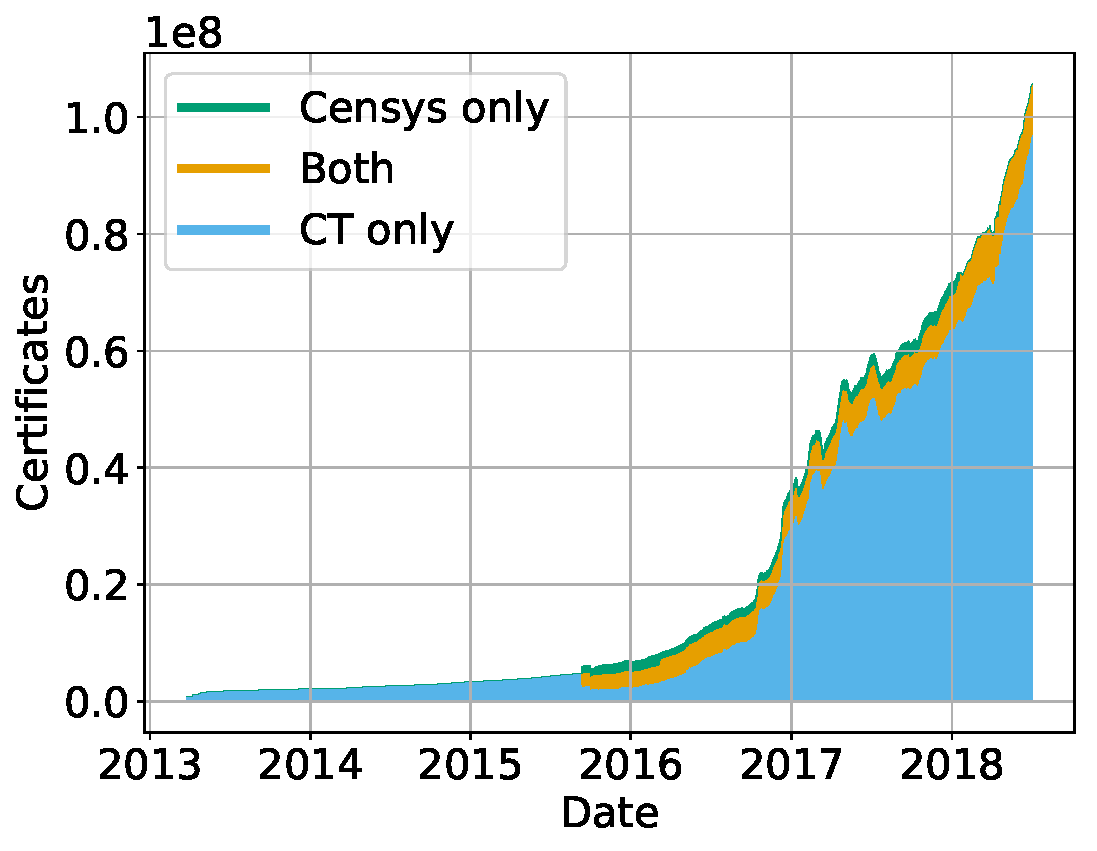
\includegraphics[width=0.33\linewidth]{fig/cert_count_valid}
    \label{fig:count:certs}
  }
  \subfloat[Names.]{
    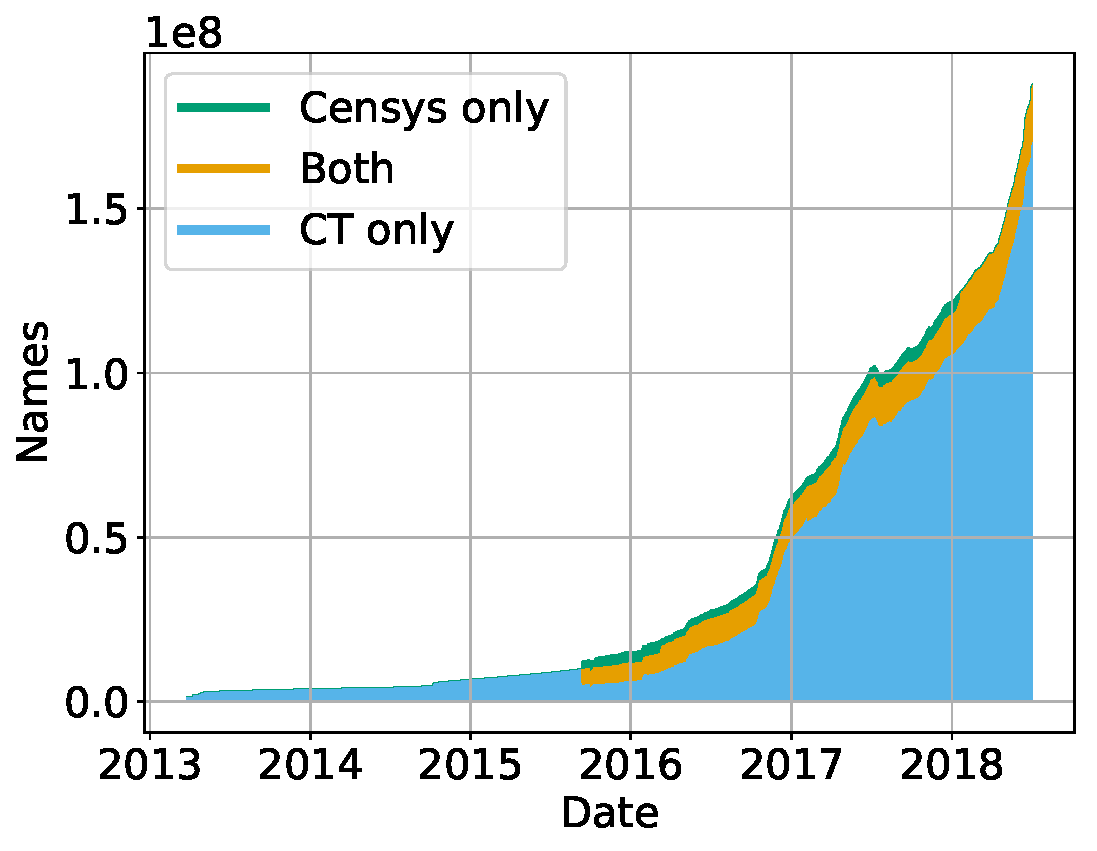
\includegraphics[width=0.33\linewidth]{fig/name_count_valid}
    \label{fig:count:names}
  }
  \subfloat[Domains.]{
    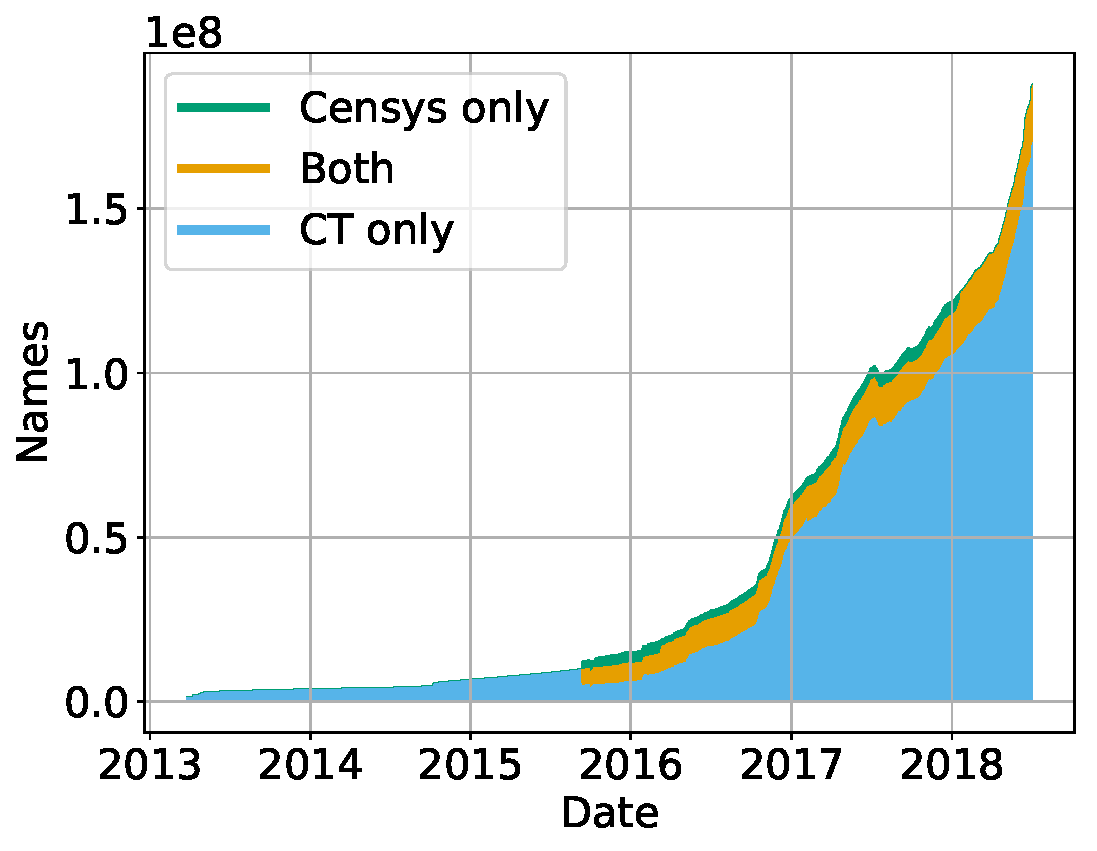
\includegraphics[width=0.33\linewidth]{fig/name_count_valid}
    \label{fig:count:domains}
  }
  \caption{Certificates, names, and domains in the Web \ac{pki} as seen by
  Censys and \ac{ct}. \steve{The domains graphic is a placeholder for now.}}
  \label{fig:count}
\end{figure*}

On each of these days, we consider an ``active set'' of certificates consisting
of all certificates that were valid on that day and had an associated
certificate chain rooted in one of the three major root certificate stores,
determined by Apple, Microsoft, or Mozilla. In the Censys dataset, because we
observed a great deal of churn (i.e., certificates disappearing and appearing in
consecutive scans), we considered a certificate as in the active set from the
time it was first observed in our data until its expiration. We then consider
the number of unique, valid domain names, which we use to build the signaling
set. \steve{Finally, we considered the unique domains (names directly under a
domain from the Public Suffix List.}

\autoref{fig:count} shows the number of each observed by Censys, \ac{ct}, and
their overlap over time. Our results show that there are far more certificates
(and consequently names and domains) observed by \ac{ct} than by Censys. To
determine whether the names seen in \ac{ct} simply never deployed HTTPS in the
wild or whether Censys was not observing certain certificates, we performed a
scan of port 443 using ZGrab~\cite{durumeric2015search} for all domain
names in \ac{ct} that were not found by Censys. We find that as of our most
recent measurement, there are \steve{XX} domain names that are accessible over
HTTPS, and that this number has seen an average growth of approximately
\steve{XX} names per day. \steve{Compare the growth rate of domains with the
growth of overall domain names, as estimated by VeriSign's quarterly Domain Name
Industry Brief, if we can get old versions.}

We also observe a surge of growth in HTTPS deployment during \steve{\emph{list
time periods here, along with events that triggered them, such as Let's Encrypt
deployment, or adoption of CT/LE by major CAs/hosting providers}}.

%As of April 2018, Google requires all newly-issued certificates to
%be logged in \ac{ct}~\cite{sleevi2017certificate}, so we expect that in time,
%the log aggregator will determine these sets solely with \ac{ct} log data.
%However, because our crawl of \ac{ct} logs (\autoref{sec:evaluation:https} shows
%that they currently contain \steve{XX\%} of known
%\steve{certificates/\acp{fqdn}}, we also used scans of the IPv4 address space
%from Censys~\cite{durumeric2015search} alongside our \ac{ct} log data to build
%\httpsset and \multicertset for our prototype. The combination of Censys and
%\ac{ct} data has been shown to encompass over 99\% of known certificates and
%\acp{fqdn}~\cite{vandersloot2016towards}.

%While previous work~\cite{vandersloot2016towards, larisch2017crlite} has
%successfully collected and used data from these sources to construct a
%near-complete view of the set of \ac{https} certificates at a given time, there
%is little data about how \ac{https} deployment has changed over time. Proxy
%measures, such as the percentage of \ac{https} connections in
%Chrome\endnote{\url{https://transparencyreport.google.com/https/overview}} or
%the number of certificates issued by Let's
%Encrypt\endnote{\url{https://letsencrypt.org/stats/}}, only provide an
%approximation of this change. In order to design \ac{name} with the appropriate
%scale of data in mind, we used data from Censys and \ac{ct} to analyze the
%change in the number of \acp{fqdn} associated with \iac{https} certificate over
%time.

%We collected certificates from Censys and \ac{ct} over a period ranging from 26
%March 2013 to 3 July 2018, though a majority of the observations are
%concentrated over the last two years. In total, we collected 58.3 billion
%entries representing 609 million distinct certificates that were either obtained
%in a \ac{tls} handshake in Censys or logged in a known good\endnote{Taken from
  %\url{https://www.certificate-transparency.org/known-logs}. A good log is a log
  %on this list that has not been disqualified or ceased operation} \ac{ct} log.
  %We then extracted all valid\endnote{A valid \ac{fqdn} has \iac{tld} that is a
  %current global \ac{tld} in ICANN, is up to 253 bytes in length overall, and
%has no label longer than 63 bytes.} \acp{fqdn} from these certificates. Because
%names and certificates appeared multiple times over these entries, we considered
%a name $N$ valid on a given day if there was at least one certificate that
%\begin{inparaenum}
%\item contained $N$ as a subject name or a subject alternative name,
%\item had been observed on or before that day, and
%\item was valid on that day (its validity period had started and not yet
  %expired).
%\end{inparaenum}

%Because HTTPS adoption trends changed during our measurement period, we focus on
%the last two years of data, from 3 July 2016 to 3 July 2018, which we show in
%\autoref{fig:certs}. There are close to 200 million distinct \acp{fqdn}
%currently associated with \iac{https} certificates. We did not find a clear
%trend that encompassed the entire range of the data, but we observe a roughly
%linear trend from April to July 2018. Specifically, the set of \acp{fqdn} that
%deploy \ac{https} grows at an average of 574,921 names per day, with $R^2=0.97$.

%\steve{Further things to explore:
  %\begin{compactitem}
  %\item How much data is captured in Censys vs \ac{ct}
  %\item Scale of \acp{fqdn} in Alexa Top 1M sites
  %\item List of names under the public suffix list
  %\item Overall trends for \ac{fqdn} growth
  %\item When names that expire reappear
  %\item Issuers/domains that don't renew before expiration
  %\end{compactitem}
%}

\subsection{Signaling Set Representation}
\label{sec:evaluation:implementation}

To justify our design decisions for our representation of the signaling set, we
used several features of our underlying set of domain names. To demonstrate the
shortcomings of other approaches, we represented this set as a Bloom filter and
as a compressed archive of strings.

Recall from \autoref{sec:design} that it is important to minimize the
size of the representation of the signaling set, as well as the latency
inflation from querying the signaling set. It is also important to ensure that
this size will not grow at an unsustainable rate as new domains deploy HTTPS.
In order to compare different approaches to representing the signaling set given
these objectives, we must examine the representations of a variety of domain
name sets with a variety of approaches.

Specifically, we compare signaling sets of various sizes using Bloom filters,
compression utilities, HTTPS Everywhere (which internally uses a set of regular
expressions) and our \ac{dafsa}-based approach. We constructed signaling sets by
selecting the set of active certificates on different days (recall that the
construction of these sets is described in \autoref{sec:evaluation:https}). We
also constructed projected future signaling sets by merging sets of domain names
over various days, up to a maximum of \steve{XX} names. For each of these sets,
we selected a sample of \steve{XX} domains \steve{representing a range of domain
name lengths} and compared the size of the representation and the distribution
of query latencies of the sample names.

\section{Signaling HTTPS Deployment}
\label{sec:signaling}

In this section, we describe the details of how we signal \ac{https} deployment
in \ac{name}.

\subsection{Data Sources}

The authors of CRLite~\cite{larisch2017crlite} observed that
Censys~\cite{durumeric2015search} and Google's set of \ac{ct}
logs\footnote{\url{https://www.certificate-transparency.org/known-logs}} have
played a critical role in making the set of all currently known \ac{tls}
certificates easily accessible. While the authors of CRLite used this knowledge
to space-efficiently store the set of all revoked certificates, in \ac{name} we
are interested in space-efficiently storing the set of all domains that have
deployed \ac{https}. We note that we can use the same data sources as CRLite
does and simply extract the set of domain names appearing in currently valid
certificates to obtain a list of all domains deploying \ac{https}.

To this end, Censys provides a scan of the entire IPv4 address space on port 443
(the default port number for \ac{https}) and the resulting \ac{tls} handshake
attempts.  \steve{(todo) We also downloaded a dump of XX \ac{ct} logs and
extracted domain names from the certificates stored at these logs.} After
extracting the data from the \steve{(update) May 18, 2017} scan results
\steve{(todo) and from the \ac{ct} log databasse}, we obtained a list of
\steve{(update) just over 69 million} domain names that take up a total of
\steve{(update) 147 MB}. This set excludes duplicate domain names as well as
common names \steve{(todo) explain in background} that are invalid DNS names.

\subsection{Approaches}

\steve{This subsection is in note form, and for now is just to summarize the
approaches I have tried.}

CRLite makes use of filter cascades (based on Bloom filters) to efficiently
store the set of all revoked certificates in around 10 MB. However, CRLite's
approach relies on having access to the set of all known certificates, which
Censys and the \ac{ct} logs can provide. While it is possible to access many of
the top-level domain zone files in DNS (including \texttt{.com}), many of the
registrars of country-specific top-level domains do not publicize their
information. Moreover, CRLite relies on the \steve{reasonable} assumption that
only a small minority of certificates will be revoked. By contrast, the rate of
\ac{https} deployment cannot be bounded by such assumptions, particular with the
advent of services such as Let's Encrypt, which has already increased the
\ac{https} deployment rate in its early stages \steve{(todo) wording}.

Constructing the signal set by simply compressing the set of \ac{https} domains
is also possible. As with most data compression algorithms, there is a clear
tradeoff between speed and compression ratio. For example, using lz4
\steve{(todo) cite} takes less than a second to compress and decompress, but
only obtains a compression ratio of 2.26 (for a compressed size of 65 MB). Using
bzip2, on the other hand, takes just over 10 seconds and has a ratio of 3.68 (40
MB compressed). Using xz took 64 seconds and produced a ratio of 4.45 (33 MB
compressed), and the best performer, zpaq (with the largest block size), took
4.5 minutes and produced a ratio of 5.88 (25 MB compressed). Unfortunately,
decompression with zpaq is slow, taking 7 minutes, and thus cannot be used to
support real-time signal set checking.

Succinct data structures provide a way for us to encode the signal set in a
space-efficient way while supporting efficient membership queries in the
succinctly encoded state. If we build a trie (also called a prefix tree) based
on the reversed domain names (capturing the highly repeated use of TLDs), we can
use the LOUDS (level order unary degree sequence) representation of the prefix
tree to efficiently encode the tree. In particular, we can represent the full
signal set in 73.3 MB. \steve{We also tried the use of minimal acyclic finite
  state automata (MAFSAs), which can represent the same information as a trie in
fewer states. However, this approach is quite slow for the number of domains we
want to represent, and there are fewer ways of efficiently encoding MAFSAs,
which in our case are effectively directed acyclic graphs with labeled edges.}

\subsection{Client Procedure}

\steve{How the client actually performs the lookup}


\begin{table}[t]
  \centering
  \caption{Size of \ac{name} signaling set on July 3, 2018 (\numnames{} names)
  with various compression approaches.}
  \begin{tabularx}{\linewidth}{|Xr|}
    \toprule
    \textbf{Representation} & \textbf{Size (MB)} \\
    Plaintext & \plaintextsize \\
    Bloom Filter (1\% FP, best-case) & \bloomlargesize \\
    Bloom Filter (0.1\% FP, best-case) & \bloommedsize \\
    Bloom Filter (0.01\% FP, best-case) & \bloomsmallsize \\
    bzip2 (100kB blocks) & \bzlargesize \\
    bzip2 (500kB blocks) & \bzmedsize \\
    bzip2 (900kB blocks) & \bzsmallsize \\
    zpaq (method 1, 16 MiB blocks) & \zpaqlargesize \\
    zpaq (method 5, 64 MiB blocks) & \zpaqmedsize \\
    zpaq (method 5, 2048 MiB blocks) & \zpaqsmallsize \\
    DAFSA & \fsalargesize \\
    DAFSA w/ path compaction & \fsamedsize \\
    DAFSA w/ path + transition compaction & \fsasmallsize \\


    %&
    %\multicolumn{2}{c|}{\textbf{Approximate Cost}}
    %& &
    %\multicolumn{2}{c|}{\textbf{Approximate Cost}}\\
    %\midrule
    %\textbf{Operation} & \textbf{Gas} & \textbf{USD} & \textbf{Operation} &
    %\textbf{Gas} & \textbf{USD} \\
    %\midrule

    %Verif.\ cert. & 31\,012 & \$0.0238 &
    %Bootstrap\,proof & 681\,731 & \$0.5232 \\
    %Register CA & 91\,400 & \$0.0701 &
    %Register DCP & 152\,579 & \$0.1171 \\
    %Update CA & 34\,656 & \$0.0266 &
    %Update DCP & 181\,226 & \$0.1391 \\

    %Order RP & 49\,024 & \$0.0376 &
    %Pre-report\,cert & 63\,951 & \$0.0491 \\
    %Create RP & 226\,892 & \$0.1741 &
    %Report cert& 149\,284 & \$0.1146 \\
    %Terminate RP & 99\,461 & \$0.0763 &
    %Send payouts & 107\,962 & \$0.0829 \\
    %Expire RP & 39\,823 & \$0.0306 &
    %CA Balance & 39\,716 & \$0.0305 \\
    %\midrule
    %\multicolumn{4}{|l}{\textbf{IKP Contract Creation}} & 1\,660\,319 & \$1.2742 \\
    \bottomrule

  \end{tabularx}
  \label{tab:op-costs}
\end{table}


As we describe in \autoref{sec:design:signaling}, we use a \ac{dafsa}-based
design of the signaling set with two optimizations over previous work. To
examine the impact of these optimizations, we perform the above comparison with
four different sets of optimizations: the minimal approach as described by
existing work~\cite{daciuk2012smaller}, our approach with transition compaction
only, our approach with path compaction only, and our approach with both
transition and path compaction. The full set of test configurations we tried
is shown in \steve{Table XX}.

Our results, shown in \steve{Figure XX}, show that Bloom filters offer fast
queries, but at the cost of either a high false positive rate or a large
representation size. On the other hand, compression utilities have no false
positives, but at the cost of either a large representation size or high query
latency. The \ac{dafsa}-based representations are at a ``sweet spot'' of these
metrics, offering a relatively small representation size as well as a relatively
low query latency. Within the \ac{dafsa}-based representations, \steve{talk
about the results here}.

%We tuned the parameters for each of these
%representations; namely, we tested the Bloom filter representation with three
%different false positive rates (10\%, 1\%, and 0.1\%), and the compressed
%archive representation with several compression utilities (gzip, bzip2, xzip,
%and zpaq) and a range of parameters specific to each utility. For each, we
%measured the size of the representation on disk, as well as the distribution of
%query latencies for a sample input set, and we compared these metrics to those
%for the \ac{dafsa}-based representation. Our results, shown in \steve{Fig. XX},
%demonstrate that \steve{the \ac{dafsa}-based representation falls on the Pareto
%frontier of size and median query latency.} Moreover, our \ac{dafsa}-based
%representation does not result in significantly user-unfriendly size or latency
%overhead.

%To justify our approach to further reduce the \ac{dafsa} size using transition
%and path compaction, we built \iac{dafsa} using the approach of prior work and
%performed several steps that reduced the size of the representation. \steve{Fig.
%XX(a)} shows the occurrences of isolated paths (length and count) and
%\steve{Fig. XX(b)} shows the size reduction, both plotted against the number of
%strings represented by the \ac{dafsa}. After applying this compaction, we show
%that the distribution of labels (\steve{Fig. XX}) as well as the distribution of
%destination states of each transition, both as absolute states (\steve{Fig.
%XX(a)} and as relative states forward or backward (\steve{Fig. XX(b)},
%justifying our use of Huffman coding for the label and destination state in each
%transition. Finally, we show selections of various connected components and
%their characteristics, along with the reduction in representation size resulting
%from applying path compaction to each component.

%Finally, to compare the coverage of HTTPS enforcement with existing tools, we
%downloaded the ruleset of HTTPS Everywhere (represented as a set of regular
%expressions) as of July 3, 2018 and measured the difference in the domain names
%represented in the ruleset and in the signaling set. The results, shown in
%\steve{Fig. XX} indicate that \steve{our signaling set covers a significantly
%larger set of domain names than HTTPS Everywhere does}.

\subsection{Connection Establishment}
\label{sec:evaluation:performance}

\begin{figure*}[thb]
  \centering
  \subfloat[vs Number of Proofs Requested]{
    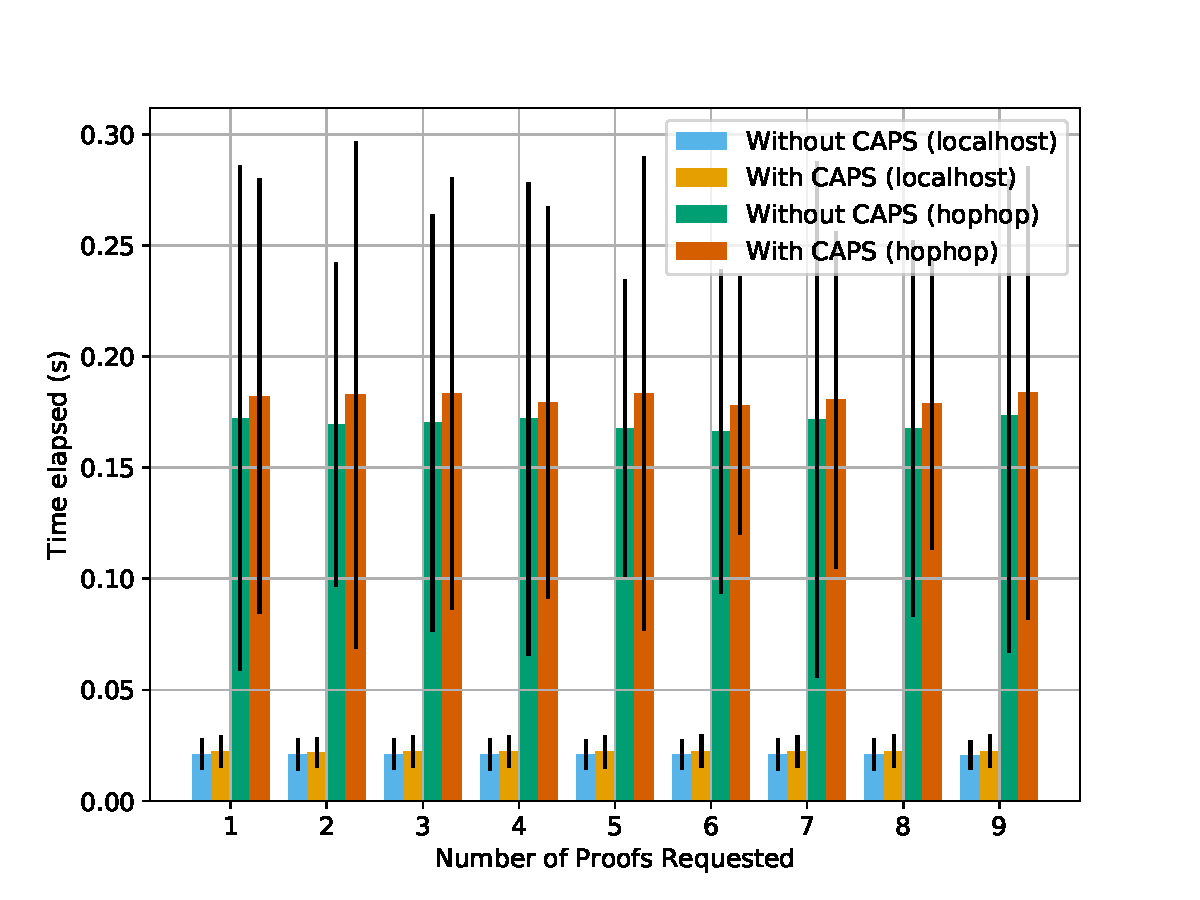
\includegraphics[width=0.24\linewidth]{fig/eval_tls_ext/0-time_elapsed_vs_num_proofs_requested}
    \label{fig:evaltlsext:numproof}
  }
  \subfloat[vs Number of Chains Sent]{
    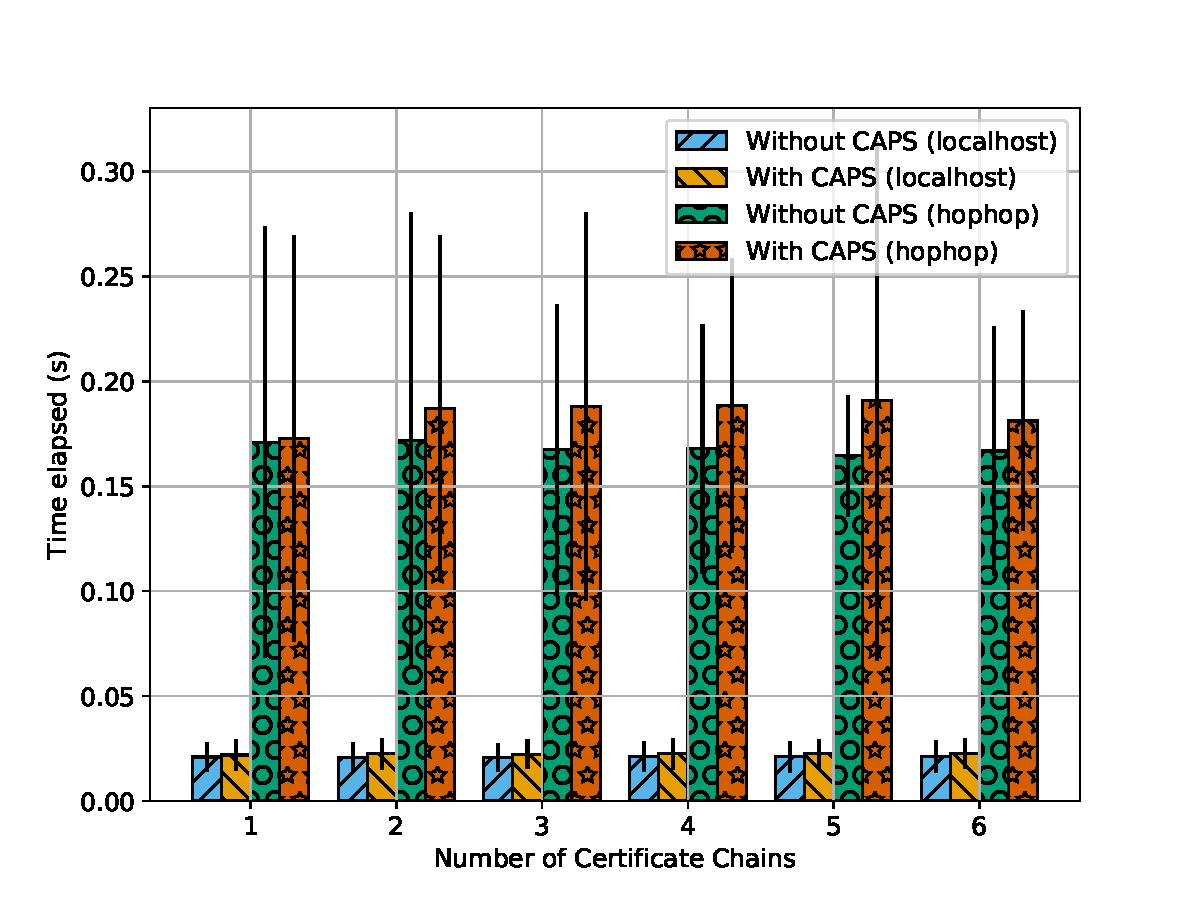
\includegraphics[width=0.24\linewidth]{fig/eval_tls_ext/1-time_elapsed_vs_num_chains_sent}
    \label{fig:evaltlsext:numchain}
  }
  \subfloat[vs Number of Certificates per Chain]{
    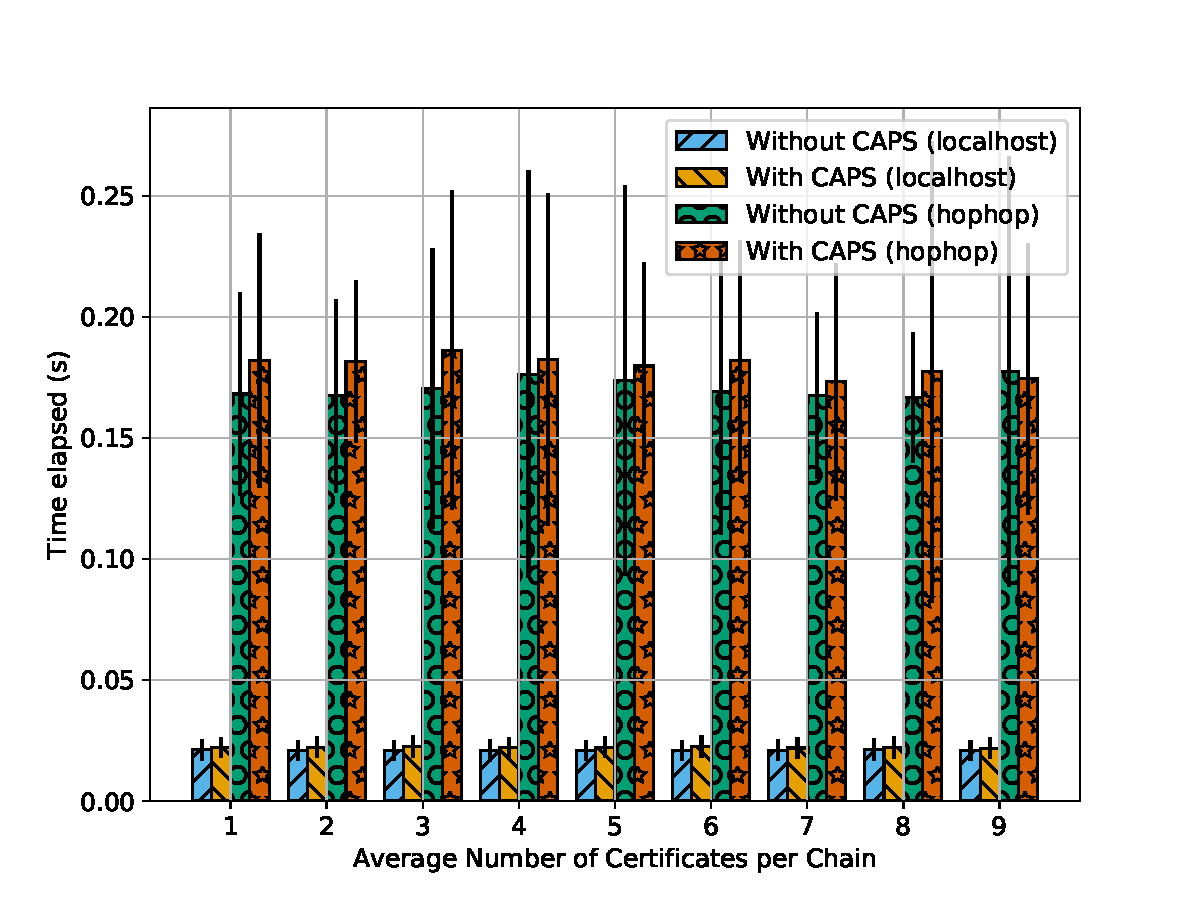
\includegraphics[width=0.24\linewidth]{fig/eval_tls_ext/2-time_elapsed_vs_num_certs_per_chain}
    \label{fig:evaltlsext:numcert}
  }
  \subfloat[vs Average Size of Chain]{
    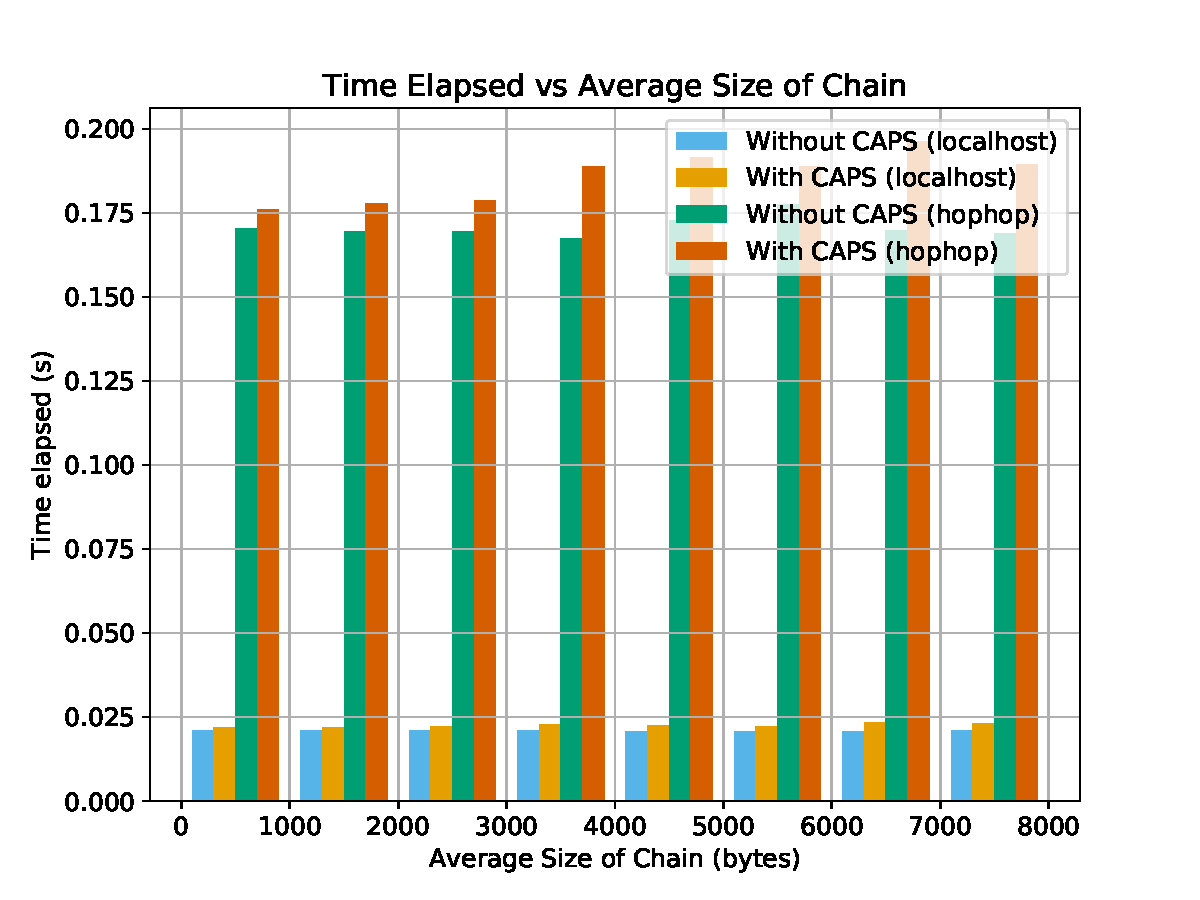
\includegraphics[width=0.24\linewidth]{fig/eval_tls_ext/3-time_elapsed_vs_avg_chain_size}
    \label{fig:evaltlsext:sizechain}
  }
  \caption{Time Elapsed during Connection Establishment \jay{TODO: Figure out how to make these readable}}
  \label{fig:evaltlsext}
\end{figure*}

% \jay{We had decided to drop the idea of a Chrome/Firefox extension in
%   favor of doing a purely curl+nginx thing}

To measure the \bryan{Need to motivate/remind} \jay{Not sure I
  understand this comment. Earlier in the section, we say ``Finally,
  we describe the performance effects of CAPS on connection
  establishment'', so this part is simply finally bringing this up,
  right?}
performance of connection establishment in \ac{name}, we
implemented the handshake as a custom \ac{tls} extension in the
OpenSSL library. For concrete evaluation of this extension, we use
nginx and curl with minor modifications to use our \ac{tls} extension.

Additionally, we constructed sample sets of domain names based
on four parameters:
\begin{inparaenum}
\item the number of proofs requested by the client (\numlas) during the ClientHello message,
\item the number of certificate chains the server \bryan{which server?} \jay{isn't this clear from the fact that we have written a TLS extension?} sends (\policy) during the ServerHello message,
\item the average number of certificates per chain, and
\item the average size of each certificate chain.
\end{inparaenum}
\jay{Number of samples collected?}
While varying each of these parameters, we measured the amount of
extra data sent in the \ac{name} handshake, and the latency of
handshake both with and without
\bryan{A bit unclear, given that most params don't apply. Need to more precisely define the baseline.}
the \ac{name} \ac{tls} extension. We
tested this both over a regular network interface
\bryan{ping latency? bandwidth?}
, by connecting to a
VPS \bryan{?} (referred to as \emph{hophop}), as well as over the local loopback
interface (referred to as \emph{localhost}) \bryan{why is the local loopback one interesting?}.

\jay{Restructure the start of this sentence}
Our results with respect to the time elapsed per \ac{tls} connection,
shown in Figure~\ref{fig:evaltlsext}, show that there is some
\bryan{be precise ; give abs + relative $\Delta$ ; small is an opinion/judgement unless you specify your comparison points}
small
latency overhead, when comparing the mean time elapsed. This appears
primarily due to
\bryan{how do you know?}
the extra data
\bryan{how much?}
sent over the network. However, since
our \ac{tls} extension does not add any extra round-trips to the
handshake, the time added is small, especially in comparison to random
measurement fluctuations, when we look at 90\% confidence intervals
\bryan{is that what the bars are? if so, say so.}
.

The extra data sent in the \ac{name} handshake is directly dependent
on the size and number of certificate chains, as well as the number of
proofs sent. In particular, the extra data sent from client to server
is 1 byte, and the extra data sent from server to client is
$(2 + (292 \times \text{\#proofs}) +
(\sum_{\text{chain}}\texttt{sizeof}(\text{chain})))$ bytes. \jay{Here,
  the chains can be serialized using whichever serialization format is
  preferred. For simplicity in implementation, we used PEM.}

%\subsection{Log Aggregator}

%To measure the resource requirements for a log aggregator, we implemented the
%log aggregator \steve{in \emph{language} on \emph{platform}}. In addition to
%retrieving signaling set data as in \autoref{sec:evaluation:https}, we also
%retrieved revocation information from \steve{CRLs, OCSP responders, and browser
%revocation lists}. We then measured the storage requirements and mapping size
%over time. \steve{Fig. XX} shows our results. \steve{Small tweaks to make to our
  %design based on these numbers. For example, we can use a NOVOMODO-like system
%to reduce the signature load for all names whose policy value doesn't change.}
